\documentclass{article} % For LaTeX2e
\usepackage{iclr-style/iclr2016_conference,times}
\usepackage{hyperref}
\usepackage{url}
\usepackage{amsmath}
\usepackage{amsfonts}
\usepackage{graphicx}
\usepackage{caption}
%\usepackage{subcaption}
\usepackage{subfig}
\usepackage{tabulary}
\usepackage{soul}
\usepackage{color}
\usepackage{xcolor}
\usepackage[bottom]{footmisc}

\captionsetup{font=small}
\newcommand{\Figref}[1]{Fig.~\ref{#1}}
\newcommand{\Secref}[1]{Sec.~\ref{#1}}
\newcommand{\Eqref}[1]{Eq.~\ref{#1}} % The '~' stops breaking and gives correct spacing
\newcommand{\Eqrefs}[2]{Eqs.~\ref{#1},~\ref{#2}}
\def\beqa#1\eeqa{\begin{eqnarray}#1\end{eqnarray}}
\newcommand{\FIXME}[1]{\textcolor{red}{[#1]}}

\newcommand{\comm}[1]{}
\newcommand{\given}{\,|\,}
\newcommand{\expectation}{\mathbb{E}}
\newcommand{\kldiv}{\mathrm{D}_{\rm KL}}
\newcommand{\klBars}{\,\|\,}
\newcommand{\sigmoid}{\boldsymbol{\sigma}}
\newcommand{\hlang}{h^{lang}}
\newcommand{\hlangall}{\boldsymbol{h^{lang}}}
\newcommand{\hdec}{h^{gen}}
\newcommand{\aalign}{{\mathit{align}}}
\newcommand{\henc}{h^{infer}}
\newcommand{\readop}{\mathit{read}}
\newcommand{\writeop}{\mathit{write}}
\newcommand{\encoder}{\mathit{LSTM}^{infer}}
\newcommand{\decoder}{\mathit{LSTM}^{gen}}
\newcommand{\canv}{c}
\newcommand{\lat}{z}
\newcommand{\vv}{{\bf v}}
\newcommand{\Lat}{Z}
\newcommand{\numSamples}{L}
\newcommand{\sampleIdx}{l}
\newcommand{\LatSample}{\tilde{Z}}
\newcommand{\icaption}{{\bf{y}}}
\newcommand{\oimage}{{\bf{x}}}
\newcommand{\post}{Q}
\newcommand{\prior}{P}
\newcommand{\loss}{\mathcal{L}}
\newcommand{\lloss}{\mathcal{L}^{z}}
\newcommand{\rloss}{\mathcal{L}^{x}}
\newcommand{\hlc}[2][yellow]{{\sethlcolor{#1}\hl{#2}}}

\definecolor{0}{RGB}{247,251,255}
\definecolor{1}{RGB}{222,235,247}
\definecolor{2}{RGB}{198,219,239}
\definecolor{3}{RGB}{158,202,225}
\definecolor{4}{RGB}{107,174,214}
\definecolor{5}{RGB}{66,146,198}

\newcommand{\hlczero}[1]{\hlc[0]{#1}}
\newcommand{\hlcone}[1]{\hlc[1]{#1}}
\newcommand{\hlctwo}[1]{\hlc[2]{#1}}
\newcommand{\hlcthree}[1]{\hlc[3]{#1}}
\newcommand{\hlcfour}[1]{\hlc[4]{#1}}
\newcommand{\hlcfive}[1]{\hlc[5]{#1}}

\newcommand{\ssmall}[1]{{\scriptsize {#1}}}


\newenvironment{myfont}{\fontfamily{[pcr]}\selectfont}{\par}
\DeclareTextFontCommand{\textmyfont}{\myfont}

\setlength{\abovecaptionskip}{5pt} % Chosen fairly arbitrarily
\setlength{\belowcaptionskip}{5pt} % Chosen fairly arbitrarily

\title{Generating Images From Captions\\ With Attention}

\author{
Elman Mansimov, Emilio Parisotto, Jimmy Lei Ba \& Ruslan Salakhutdinov\\
Department of Computer Science\\
University of Toronto\\
Toronto, Ontario, Canada\\
\texttt{\{emansim,eparisotto,rsalakhu\}@cs.toronto.edu}, \texttt{jimmy@psi.utoronto.ca}
}

\newcommand{\fix}{\marginpar{FIX}}
\newcommand{\new}{\marginpar{NEW}}

\begin{document}

\maketitle

\begin{abstract}
%\vspace{-0.3cm}
Motivated by the recent progress in generative models, we introduce a model that generates images from natural language descriptions. The proposed model iteratively draws patches on a canvas, while attending to the relevant words in the description. After training on Microsoft COCO, we compare our models with several baseline generative models on image generation and retrieval tasks. We demonstrate that our model produces higher quality samples than other approaches and generates images with novel scene compositions corresponding to previously unseen captions in the dataset. 
\end{abstract}

\section{Introduction}
%\vspace{-0.2cm}
Statistical natural image modelling remains a fundamental problem in computer vision and image understanding. 
The challenging nature of this task has motivated recent approaches to exploit the inference and generative capabilities of deep neural networks.
Previously studied deep generative models of images often defined distributions that were restricted to being either unconditioned or conditioned on classification labels. In real world applications, however, images rarely appear in isolation as they are often accompanied by unstructured textual descriptions, such as on web pages and in books. 
The additional information from these descriptions could be used to simplify the image modelling task. Moreover, learning generative models conditioned on text also allows a better understanding of the generalization performance of the model, as we can create textual descriptions of completely new scenes not seen at training time. 

%There are two primary directions in learning a generative model of image and text.  
There are numerous ways to learn a generative model over both image and text modalities. One approach is to learn a generative model of text conditioned on images, known as caption generation
%A significant amount of recent work has focused on generating captions from images
\citep{karpathy_captions}, \citep{vinyals_captions}, \citep{xu_captions}. These models take an image descriptor and generate unstructured texts using a recurrent decoder. In contrast, we will explore models that condition in the opposite direction, i.e. taking textual descriptions as input and using them to generate relevant images.
%By contrast, learning a generative model for image and text may also be studied by generating images correctly interpreting the text description. 
Generating high dimensional realistic images from their descriptions 
%is a more difficult approach that 
combines the two challenging components of language modelling and image generation, and can be considered to be more difficult than caption generation. %Namely, the model has to capture the semantic meaning expressed in the description and then use that knowledge to generate pixel intensities of the image.

In this paper, we illustrate how sequential deep learning techniques can be used to build a conditional probabilistic model over natural image space effectively. By extending the Deep Recurrent Attention Writer (DRAW) \citep{gregor_draw}, our model iteratively draws patches on a canvas, while attending to the relevant words in the description. Overall, the main contributions of this work are the following: we introduce a conditional alignDRAW model, a generative model of images from captions using a soft attention mechanism. The images generated by our alignDRAW model are refined in a post-processing step by a deterministic Laplacian pyramid adversarial network \citep{denton_lapgan}. We then illustrate how our method, learnt on Microsoft COCO \citep{mscoco}, generalizes to captions describing novel scenarios that are not seen in the dataset (Figure~\ref{fig:genimages4}). 

\section{Related Work}

\begin{figure}[!t]
\captionsetup[subfigure]{labelformat=empty}
\vspace{-0.3cm}
\begin{center}
\subfloat[A stop sign is flying in blue skies.
]{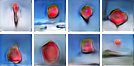
\includegraphics[width=0.23\textwidth]{figures/new/a-stop-sign-is-flying-in-blue-skies-sharp.png}}\quad
%
\subfloat[A herd of elephants flying in the blue skies.
]{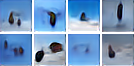
\includegraphics[width=0.23\textwidth]{figures/new/a-herd-of-elephants-flying-in-the-blue-skies-sharp.png}}\quad
%
\subfloat[A toilet seat sits open in the grass field.
]{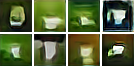
\includegraphics[width=0.23\textwidth]{figures/new/a-toilet-seat-sits-open-in-the-grass-field-sharp.png}}\quad
%
\subfloat[A person skiing on sand clad vast desert.
]{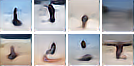
\includegraphics[width=0.23\textwidth]{figures/new/a-person-skiing-on-sand-clad-vast-desert-sharp.png}}\quad
%
\end{center}
\caption{Examples of novel scene compositions.}
\label{fig:genimages4}
\vspace{-0.3cm}
\end{figure}

Deep Neural Networks have achieved significant success in various tasks such as image recognition \citep{krizhevsky_imagenet} and speech transcription \citep{graves_speech}. 
While most of the recent success has been achieved by discriminative models, generative models have not yet enjoyed the same level of success. Most of the previous work in generative models has focused on variants of Boltzmann Machines \citep{smolensky_rbm}, \citep{russ_dbm} and Deep Belief Networks \citep{hinton_dbn}. While these models are very powerful, each iteration of training requires a computationally costly step of MCMC to approximate an intractable normalization constant, making it difficult to scale them to large datasets.

\cite{kingma_vae} have introduced the Variational Auto-Encoder (VAE) which can be seen as a neural network with continuous latent variables. The encoder is used to approximate a posterior distribution and the decoder is used to stochastically reconstruct the data from latent variables. The model's efficient inference and learning procedures allow it to scale to large datasets. 
\cite{gregor_draw} introduced the Deep Recurrent Attention Writer (DRAW), extending the VAE approach by incorporating a novel differentiable attention mechanism which significantly improved performance.% as well as quality of generated samples.
%While most of the samples from VAE and DRAW models resemble a clear structure of objects, the generated images are blurry most of the time.

Generative Adversarial Networks (GANs) \citep{goodfellow_gan} are another type of generative models that use noise-contrastive estimation \citep{gutmann_nce} to avoid calculating an intractable normalization constant. The model consists of a generator that generates samples using a uniform distribution and a discriminator that discriminates between real and generated images. 
Both networks can be seen as playing a game against each other, where the generator tries to produce samples that look real and the discriminator tries not to be fooled by the generator. 
Recently, \cite{denton_lapgan} have scaled those models by training conditional GANs at each level of a Laplacian pyramid of images. 
%While their model has generated sharp looking samples, the generated images have lacked a clear structure. 
%Compared to other mentioned generative models, GANs are more unstable and are harder to train.

While all of the previous work has been focused on unconditional models or models conditioned on labels, to the best of our knowledge this paper is the first to introduce a generative model of images conditioned on captions.

\section{Model}
\label{sec:model}
Our proposed model 
defines a generative process of images conditioned on captions. In particular, captions are represented as a sequence of consecutive words and images are represented as a sequence of patches drawn on a canvas $c_t$ over time $t=1,...,T$. Our model can be viewed as a part of the sequence-to-sequence framework \citep{ilya_mt,cho_mt,nitish_video}.
%Our proposed model can be viewed as a part of sequence-to-sequence framework \citep{ilya_mt}, \citep{cho_mt}, \citep{nitish_video} where captions are represented as a sequence of consecutive words and images are represented as a sequence of patches drawn on canvas over time $t=1,...,T$. Let $\icaption$ be the input caption, consisting of $N$ words $y_{1}, y_{2}, ..., y_{n}$ and $\oimage$ be the image corresponding to that caption.

\subsection{Language Model: the Bidirectional Attention RNN}
\label{sec:lang}
Let $\icaption$ be the input caption, represented as a sequence
of 1-of-K encoded words 
${\bf y} = \{y_{1}, y_{2}, ..., y_{N}\}$, 
where $K$ is the size of the vocabulary and $N$ is the length of the sequence.
%and $\oimage$ be the output image. 
We obtain the caption sentence representation by first 
transforming each word $y_{i}$ to an $m$-dimensional 
vector representation $\hlang_{i}$, $i=1,..,N$ using the Bidirectional RNN. In a Bidirectional RNN, the two LSTMs~\citep{hochreiter_lstm} with \textit{forget} gates 
\citep{gers_forget} process the input sequence from both forward and backward directions. The Forward LSTM computes the sequence of forward hidden states $[\overrightarrow{h}^{lang}_{1}, \overrightarrow{h}^{lang}_{2}, ..., \overrightarrow{h}^{lang}_{N}]$ , whereas the Backward LSTM computes the sequence of backward hidden states $[\overleftarrow{h}^{lang}_{1}, \overleftarrow{h}^{lang}_{2}, ..., \overleftarrow{h}^{lang}_{N}]$. 
These hidden states are then concatenated together 
into the sequence $\hlangall = [\hlang_{1}, \hlang_{2}, ..., \hlang_{N}]$, 
with $\hlang_{i} = [\overrightarrow{h}^{lang}_{i}, \overleftarrow{h}^{lang}_{i}], 1\leq i\leq N$.


\begin{figure}[t!]
\captionsetup[subfigure]{labelformat=empty}
\begin{center}
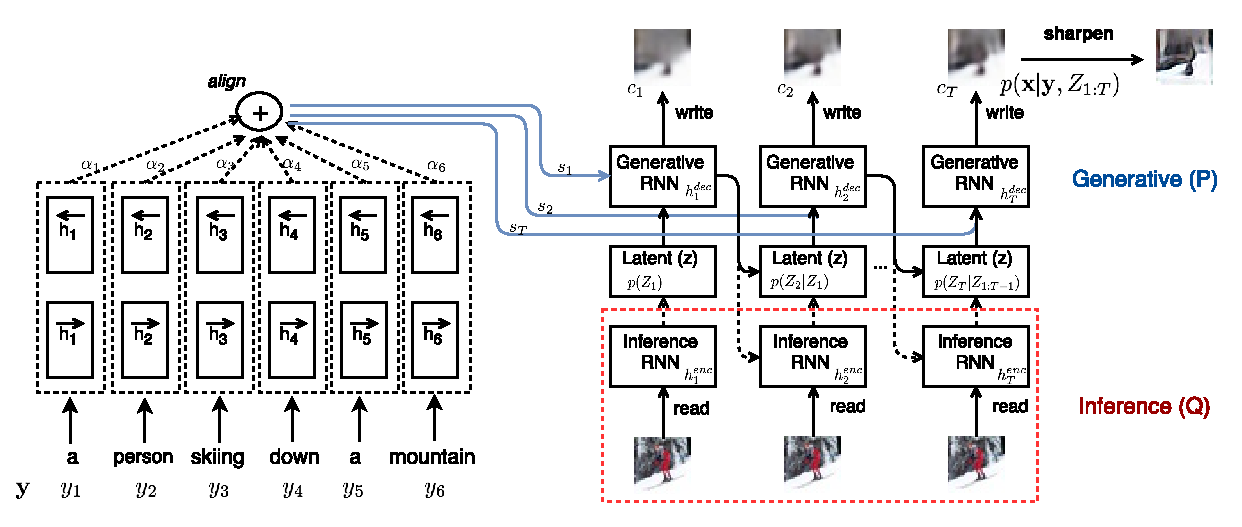
\includegraphics[width=0.99\textwidth]{figures/alignDrawAnnotated.pdf}\quad
%
\end{center}
\caption{The diagram shows our model learns to draw images by learning an alignment of input captions and generating canvas. The details are explained in Section \ref{sec:model}.}
\label{fig:figmodel}
\vspace{-0.3cm}
\end{figure}



\subsection{Image Model: the Conditional DRAW Network}

To generate an image $\oimage$ conditioned on the caption information $\bf{y}$, 
we extended the DRAW network~\citep{gregor_draw} to include caption representation $\hlangall$ at each step, as shown in \Figref{fig:figmodel}. 
The conditional DRAW network is a stochastic recurrent neural network (LSTM) that consists of a 
sequence of latent variables $\Lat_t \in \mathbb{R}^D$, $t=1,..,T$, where the output is accumulated over all $T$ time-steps.

Unlike the original DRAW network where latent variables are independent 
spherical Gaussians $\mathcal{N}(0, I)$, the latent variables in the proposed alignDRAW model have their mean and variance depend on the previous recurrent hidden states $\hdec_{t-1}$, except for $\lat_1 \sim \prior(\Lat_1) = \mathcal{N}(0, I)$.  
Namely, the mean and variance of the prior distribution over $\Lat_t$ are parameterized by: 
\begin{align}
\lat_t \sim \prior(\Lat_t|\Lat_{1:t-1}) &= \mathcal{N}\bigg(\mu(\hdec_{t-1}), \sigma(\hdec_{t-1})\bigg), \nonumber \\
\mu(\hdec_{t-1}) &= \tanh(W_{\mu}\hdec_{t-1}),\nonumber \\
\sigma(\hdec_{t-1}) &= \exp\big(\tanh(W_{\sigma}\hdec_{t-1})\big), \nonumber 
\end{align}
where $W_{\mu} \in \mathbb{R}^{D \times n}$, $W_{\sigma} \in \mathbb{R}^{D \times n}$ are 
the learned model parameters, and $n$ is the dimensionality of $\hdec_{t}$,
the hidden state of the generative LSTM. 
Similar to \cite{bachman_sdm}, we have observed that 
the model performance is improved by including dependencies between latent variables. 

Formally, an image is generated by iteratively computing the following set of 
equations for $t=1,...,T$ (see Figure~\ref{fig:figmodel}), with $\hdec_0$ and $c_0$
initialized to learned biases:
\begin{align}
\label{eq:x_hat}
\lat_t &\sim \prior(\Lat_t|\Lat_{1:t-1}) = \mathcal{N}\bigg(\mu(\hdec_{t-1}), \sigma(\hdec_{t-1})\bigg),\\
s_{t} &= align(\hdec_{t-1}, \hlangall), \\
\label{eq:decoder}
\hdec_t &= \decoder(\hdec_{t-1}, [z_t, s_{t}]), \\
\label{eq:writeop}
\canv_t &= \canv_{t-1} + \writeop(\hdec_t), \\
\tilde{\oimage} &\sim P(\oimage\given\icaption, \Lat_{1:T}) = \prod_i P(x_i\given\icaption, \Lat_{1:T}) = \prod_i \textrm{Bern}(\sigmoid(\canv_{T,i})). 
\label{eq:write}
\end{align}
The $align$ function is used to compute the alignment between the input caption and intermediate image generative steps \citep{bahdanau_mt}. 
Given the caption representation from the language model, $\hlangall = [\hlang_{1}, \hlang_{2}, ..., \hlang_{N}]$, the $align$ operator outputs a dynamic sentence representation $s_t$ at each step through a weighted sum using alignment probabilities 
$\alpha_{1...N}^{t}$:
\beqa
s_t=align(\hdec_{t-1}, \hlangall) = 
\alpha_{1}^{t}\hlang_{1} + \alpha_{2}^{t}\hlang_{2} + ... + \alpha_{N}^{t}\hlang_{N}.
\nonumber 
\eeqa
The corresponding alignment probabilities $\alpha_{1...N}^{t}$ are obtained using the caption representation $\hlangall$ and the hidden state of the generative model $\hdec_{t-1}$, by first calculating energies using a $\tanh$ perceptron scaled by vector $\vv$
and then normalizing them: %, as in \citep{bahdanau_mt}:
\beqa
\alpha_{k}^{t}=\frac{\exp(\vv^{\top}\tanh(U\hlang_{k} + W\hdec_{t-1} + b)}{\sum_{j=1}^{N}
\exp(\vv^{\top}\tanh(U\hlang_{j} + W\hdec_{t-1} + b)},
\nonumber 
\eeqa
where $U \in \mathbb{R}^{d \times m}$, $W \in \mathbb{R}^{d \times n}$ and 
$b \in \mathbb{R}^{d \times 1} $ are the learned model parameters of the alignment model. 

The $\decoder$ function of \Eqref{eq:decoder} 
is defined by the LSTM network with \textit{forget} gates 
\citep{gers_forget} at a single time-step. To generate the next 
hidden state $\hdec_t$, 
the decoder $\decoder$ takes the previous hidden state $\hdec_{t-1}$ and
combines it with the input from both the latent sample $z_t$ and 
sentence representation $s_t$, where
$[v_1, v_2]$ denotes the concatenation of $v_1$ and $v_2$ into the single vector.

The output of the decoder $\hdec_t$ is then passed through the $\writeop$ operator 
which is added to a cumulative canvas matrix $c_t$ (\Eqref{eq:writeop}). 
\FIXME{Jimmy, could you put more about the write operator}. 
The $\writeop$ operator
applies an array of Gaussian filters on the patch, placing 
it on the canvas $c_t$ with smoothly varying location and zoom (same as 
defined in \citep{gregor_draw}). 

Finally, each pixel $\canv_{T,i}$ from the final canvas $\canv_T$ is transformed using a sigmoid function $\sigmoid$ to produce a conditional Bernoulli 
distribution with the mean vector $\sigmoid(\canv_{T})$ over the image pixels 
$\oimage$ given the latent variables $\Lat_{1:T}$ and the input caption $\icaption$,



\subsection{Learning}

%The model is learned by the modified version of Stochastic Gradient Variation Bayes (SGVB) algorithm introduced by \cite{kingma_vae}. 
The model is trained to maximize a variational lower bound $\loss$ 
on the marginal likelihood of the correct image $\oimage$ given the input caption $\icaption$:
\beqa
\loss = \sum_{\Lat}Q(\Lat\given\oimage,\icaption)\left(\log P(\oimage\given\icaption, \Lat) - \kldiv\left(Q(\Lat\given\oimage,\icaption)\klBars 
  P(\Lat)\right)\right) \le \log P(\oimage\given\icaption).
\eeqa
%The posterior inference over the latent variables $\Lat_{1:T}$ is approximated using the inference RNN. 
Similar to the DRAW model, the inference recurrent network 
produces an approximate posterior $Q(\Lat_{1:T}\given\oimage,\icaption)$ via a $\readop$ operator, which reads a patch from image using an array of Gaussian filters (inverse of $\writeop$), over the training image at each step. Specifically, 
\begin{align}
\label{eq:x_hat}
\hat{\oimage}_t &= \oimage-\sigmoid(\canv_{t-1}),\\
\label{eq:read}
r_t &= \readop(\oimage_t, \hat{\oimage}_t, \hdec_{t-1}),\\
\henc_t &= \encoder(\henc_{t-1}, [r_t, \hdec_{t-1}]),\\
\post(\Lat_t|\oimage,\icaption,\Lat_{1:t-1}) &= \mathcal{N}\left(\mu(\henc_t), \sigma(\henc_t)\right),
\end{align}
%The $\loss$ is decomposed into the latent loss $\lloss$ and the reconstruction loss $\rloss$. 
%The reconstruction loss $\rloss$ equals to $\frac{1}{L}\sum_{l=1}^{L}(log\,p(x_{t}|y,z)$ where $L$ is the number of samples used during training, which was set to $1$ in our experiments.
%The latent loss $\lloss$ is a negative sum of Kullback--Leibler divergence terms between distribution $\post(\Lat_t|\henc_t)$ and some prior distribution ${\prior(\Lat_t)}$ over time $t=1,...,T$, which can be seen as a regularization term. 
%Since the prior distribution at time $t$ is dependent on the sufficient statistics of the prior distribution at time $t-1$. Namely, the mean and variance of $\prior(\Lat_t)$ depends on the $\hdec_{t-1}$. 
%\begin{align}
%\mu_{t}^{prior} &= tanh(W_{\mu}\hdec_{t-1})\\
%\sigma_{t}^{prior} &= exp(tanh(W_{\sigma}\hdec_{t-1})) 
%\end{align}
where $\hat{\oimage}$ is the \textit{error} image and $\henc_0$ is initialized to the learned bias $b$. 
Note that the inference encoder $\encoder$ 
takes both the output
of the $\readop$ operator $r_t$, which depends on the original input image $\oimage$,
and the previous state of the 
generative decoder $\hdec_{t-1}$, which depends on the latent sample history $z_{1:t-1}$ and 
caption representation $s_t$ (see \Eqref{}). 
Hence, the approximate posterior $Q$ will depend on the input image $\oimage$,
the corresponding caption $\icaption$, and the latent history $\Lat_{1:t-1}$.     
  

The terms in the variational lower bound are rearranged using the law of total expectation. Therefore, the objective function $\loss$ is calculated as follows:
\begin{align}
\label{eq:loss}
\loss =  &\expectation_{Q(\Lat_{1:T}\given\icaption,\oimage)}\left[ \log p(\oimage\given\icaption,\Lat_{1:T}) - \sum_{t=2}^T\kldiv\left(\post(\Lat_t\given\Lat_{t-1},\icaption,\oimage)\klBars\prior(\Lat_t\given\Lat_{t-1},\icaption)\right) \right] \nonumber \\& - \kldiv\left(\post(\Lat_1\given\oimage)\klBars\prior(\Lat_1)\right).
\end{align}
The expectation can be approximated by $\numSamples$ Monte Carlo samples $\LatSample_{1:T}$ from $\post(\Lat_{1:T}\given\icaption, \oimage)$:
\begin{align}
\label{eq:loss_mc}
\loss \approx  &\frac{1}{\numSamples}\sum_{\sampleIdx=1}^\numSamples\left[ \log p(\oimage\given\icaption,\LatSample^\sampleIdx_{1:T}) - \sum_{t=2}^T\kldiv\left(\post(\Lat_t\given\LatSample^\sampleIdx_{t-1},\icaption,\oimage)\klBars\prior(\Lat_t\given\LatSample^\sampleIdx_{t-1},\icaption)\right) \right] \nonumber \\& - \kldiv\left(\post(\Lat_1\given\oimage)\klBars\prior(\Lat_1)\right).
\end{align}
We used only one sample during training for all our experiments.
\comm{
\begin{align}
\loss &= -\sum_{t=1}^{T}D_{KL}(\post(\Lat_t|\henc_t,s_{t-1})\,||\,\prior(\Lat_t)) + \frac{1}{L}\sum_{l=1}^{L}log\,p(x_{t}|y,z)\\
&=
\frac{1}{2}\sum_{t=1}^{T}(1 - 2\,log\,\sigma_{t}^{prior} + 2\,log\,\sigma_{t} - \frac{\exp(2\,log\,\sigma_{t}) + (\mu_{t} - \mu_{t}^{prior})^{2}}{\exp(2\,log\,\sigma_{t}^{prior})}) + \frac{1}{L}\sum_{l=1}^{L}log\,p(x_{t}|y,z)
\end{align}
}

\subsection{Generating Images from Captions}

\begin{figure}[!t]
\captionsetup[subfigure]{labelformat=empty}
\begin{center}
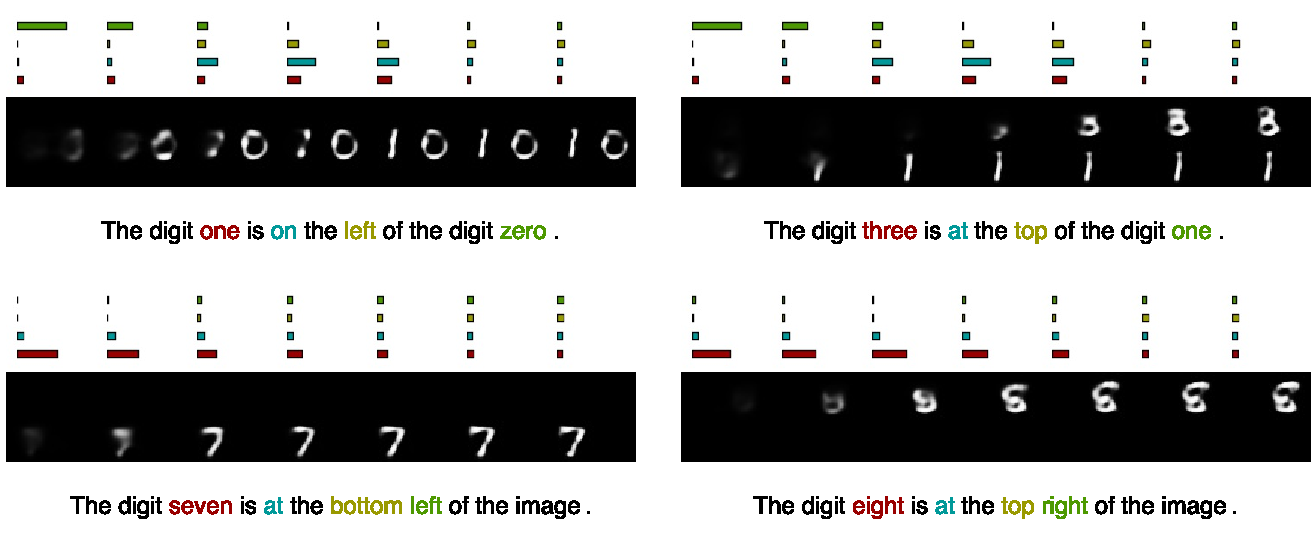
\includegraphics[width=0.99\textwidth]{figures/new/mnist/test3.pdf}\quad
%
\end{center}
\caption{Examples of generating $60 \times 60$ MNIST images corresponding to respective captions. The captions on the \textbf{left column} were part of the training set. The digits described in the captions on the \textbf{right column} were hidden during training for the respective configurations.}
\label{fig:figmnist}
\vspace{-0.3cm}
\end{figure}

During the image generation step, we discard the inference network and instead sample from the prior distribution. 
Due to the blurriness of samples generated by the DRAW model, we perform an additional post processing step where we use a 
adversarial network trained on residuals of a Laplacian pyramid conditioned on the skipthought representation \citep{kiros_skipthought} of the captions 
to sharpen the generated images, similar to \citep{denton_lapgan}. By fixing the prior of the adversarial generator to its mean, it gets treated as a deterministic neural network that allows us to define the conditional data term in Eq. (\ref{eq:loss}) on the sharpened images and calculate the lower bound accordingly. Additionally, we noticed that sampling from the mean of the uniform distribution generated samples with less noise than if we had otherwise sampled from the uniform distribution itself.  

%\newpage
\section{Experiments}
\subsection{MNIST With Captions}
As a first experiment, we trained our proposed model on the MNIST dataset with artificial captions. Either one or two digits from the MNIST training dataset were placed on a $60 \times 60$ blank image. One digit was placed in one of the four (top-left, top-right, bottom-left or bottom-right) corners of the image. Two digits were either placed horizontally or vertically in nonoverlapping fashion. 
While many generative models were trained on the binarized version of the MNIST dataset, we trained directly on pixel intensities with a binary cross-entropy cost function.

The generated images together with the attention alignments are displayed in Figure~\ref{fig:figmnist}. The model correctly displayed the specified digits at the described positions and even managed to generalize reasonably to the configurations that were never present during training. 
In the case of generating two digits, the model attended to the digit in the caption it was drawing at that particular time-step while completely ignoring the other digit. 
Similarly, when generating one digit the model attended to the digit in the caption during the whole generation process. However in both cases, the model placed small attention values on the words describing the position of digits in the images.

\subsection{Microsoft COCO}

\begin{figure}[!t]
\captionsetup[subfigure]{labelformat=empty}
\vspace{-0.3cm}
\begin{center}
\subfloat[A \underline{yellow} school bus parked in a parking lot.
]{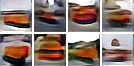
\includegraphics[width=0.23\textwidth]{figures/new/a-yellow-school-bus-parked-in-a-parking-lot-sharp.png}}\quad
%
\subfloat[A \underline{red} school bus parked in a parking lot.
]{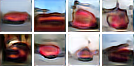
\includegraphics[width=0.23\textwidth]{figures/new/a-red-school-bus-parked-in-a-parking-lot-sharp.png}}\quad
%
\subfloat[A \underline{green} school bus parked in a parking lot.
]{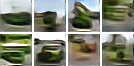
\includegraphics[width=0.23\textwidth]{figures/new/a-green-school-bus-parked-in-a-parking-lot-sharp.png}}\quad
%
\subfloat[A \underline{blue} school bus parked in a parking lot.
]{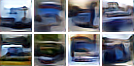
\includegraphics[width=0.23\textwidth]{figures/new/a-blue-school-bus-parked-in-a-parking-lot-sharp.png}}\quad
\\
%
\subfloat[\underline{The decadent chocolate} \underline{desert} is on the table.
]{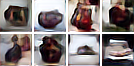
\includegraphics[width=0.23\textwidth]{figures/new/the-decadent-chocolate-dessert-is-on-the-table-sharp.png}}\quad
%
\subfloat[\underline{A bowl of bananas} is on the table.
]{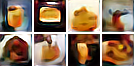
\includegraphics[width=0.23\textwidth]{figures/new/a-bowl-of-bananas-is-on-the-table-sharp.png}}\quad
%
\subfloat[A vintage photo of a \underline{cat}.
]{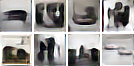
\includegraphics[width=0.23\textwidth]{figures/new/a-vintage-photo-of-a-cat-sharp.png}}\quad
%
\subfloat[A vintage photo of a \underline{dog}.
]{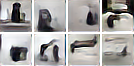
\includegraphics[width=0.23\textwidth]{figures/new/a-vintage-photo-of-a-dog-sharp.png}}\quad
%
\end{center}
\caption{\textbf{Bottom}: Examples of changing the object while keeping the caption fixed. \textbf{Top}: Examples of changing the color while keeping the caption fixed.}
\label{fig:genimages3}
%\vspace{-0.3cm}
\end{figure}

Microsoft COCO \citep{mscoco} is a very large dataset of roughly 83k images, each annotated with 5 captions. The rich collection of images with a wide variety of styles, backgrounds and objects makes the task of learning a good generative model 
%conditioned on a caption 
very challenging. For consistency with related work on caption generation, we used only the first five captions when training and evaluating our model. 
The images were resized to $32 \times 32$ dimension for consistency with other tiny image datasets \citep{krizhevsky_cifar}. In the following subsections, we analyzed both the qualitative and quantitative aspects of our model as well as compared its performance with that of other, related generative models\footnote{To see more generated images, go to \url{http://www.cs.toronto.edu/~emansim/cap2im.html}}.

\subsubsection{Analysis of Generated Images}
The main goal of this work is to learn a model that can understand the semantic meaning expressed in the textual descriptions of images, such as the properties of objects, the relationships between them, etc. and then use that knowledge to generate relevant images. To examine the understanding of our model, we wrote a set of captions inspired by the COCO dataset and changed some words in the captions to see whether the model made the relevant changes in the generated samples.

First, we wanted to see whether the model understood one of the most basic properties of any object, the color. In Figure~\ref{fig:genimages3}, we generated images of school buses with four different colors: yellow, red, green and blue. Although, there are images of buses with different colors in the training set, all mentioned school buses are specifically colored yellow. Despite that, the model managed to generate images of an object that is visually reminiscent of a school bus that is painted with the specified color.

Apart from changing the colors of objects, we were curious whether changing the background of the scene described in a caption would result in the appropriate changes in the generated samples. The task of changing the background of an image is somewhat harder than just changing the color of an object because the model will have to make alterations over a wider visual area. Nevertheless, as shown in Figure~\ref{fig:genimages2} changing the skies from blue to rainy in a caption as well as changing the grass type from dry to green in another caption resulted in the appropriate changes in the generated image.

Despite a large number of ways of changing colors and backgrounds in descriptions, in general we found that the model made appropriate changes as long as some similar pattern was present in the training set. However, the model struggled when the visual difference between objects was very small, such as when the objects have the same general shape and color. In Figure~\ref{fig:genimages3}, we demonstrate that when we swap two objects that are both visually similar, for example cats and dogs, it is difficult to discriminate solely from the generated samples whether it is an image of a cat or dog, even though we might notice an animal-like shape. This highlights a limitation of the model in that it has difficulty modelling the fine-grained details of objects.

As a test of model generalization, we tried generating images corresponding to captions that describe scenarios that are highly unlikely to occur in real life. These captions describe a common object doing unusual things 
or set in a strange location.
%that are impossible in the real world. 
%considering the physics of real world. 
Even though some of these scenarios may never happen in real life, it is very easy for humans to imagine the corresponding scene. Nevertheless, as you can see in Figure~\ref{fig:genimages4}, the model managed to generate reasonable images.  

\subsubsection{Analysis of Attention}
\begin{figure}[!t]
\captionsetup[subfigure]{labelformat=empty}
%\vspace{-0.5cm}
\begin{center}
\subfloat[]{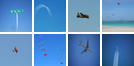
\includegraphics[width=0.23\textwidth]{figures/new/a-very-large-commercial-plane-flying-in-blue-skies-closest.png}}\quad
%
\subfloat[]{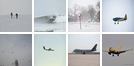
\includegraphics[width=0.23\textwidth]{figures/new/a-very-large-commercial-plane-flying-in-rainy-skies-closest.png}}\quad
%
\subfloat[]{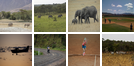
\includegraphics[width=0.23\textwidth]{figures/new/a-herd-of-elephants-walking-across-a-dry-grass-field-closest.png}}\quad
%
\subfloat[]{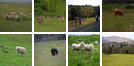
\includegraphics[width=0.23\textwidth]{figures/new/a-herd-of-elephants-walking-across-a-green-grass-field-closest.png}}\\
\vspace{-0.45cm}
%
\subfloat[A very large commercial plane flying in \underline{blue} skies.
]{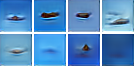
\includegraphics[width=0.23\textwidth]{figures/new/a-very-large-commercial-plane-flying-in-blue-skies-sharp.png}}\quad
%
\subfloat[A very large commercial plane flying in \underline{rainy} skies.
]{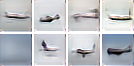
\includegraphics[width=0.23\textwidth]{figures/new/a-very-large-commercial-plane-flying-in-rainy-skies-sharp.png}}\quad
%
\subfloat[A herd of elephants walking across a \underline{dry} grass field.
]{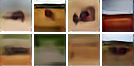
\includegraphics[width=0.23\textwidth]{figures/new/a-herd-of-elephants-walking-across-a-dry-grass-field-sharp.png}}\quad
%
\subfloat[A herd of elephants walking across a \underline{green} grass field.
]{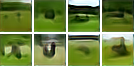
\includegraphics[width=0.23\textwidth]{figures/new/a-herd-of-elephants-walking-across-a-green-grass-field-sharp.png}}\quad
%
\end{center}
\caption{\textbf{Bottom}: Examples of changing the background while keeping the caption fixed. \textbf{Top}: The respective nearest training images based on pixel-wise L2 distance. The nearest images from the training set also indicate that the model was not simply copying the patterns it observed during the learning phase.}
\label{fig:genimages2}
%\vspace{-0.3cm}
\end{figure}

After flipping sets of words in the captions, we were curious to see which words the model attended to when generating images. It turned out that during the generation step, the model mostly focused on the specific words (or nearby words) that carried the main semantic meaning expressed in the sentences. The attention values of words in sentences helped us interpret the reasons why the model made the changes it did when we flipped certain words. For example, in Figure~\ref{fig:diffmodels} we can see that when we flipped the word ``desert'' to ``forest'', the attention over words in the sentence did not change drastically. This suggests that, in their respective sentences, the model looked at ``desert'' and ``forest'' with relatively equal probability, and thus made the correct changes. In contrast, when we swap words ``beach'' and ``sun'', we can see a drastic change between sentences in the probability distribution over words. By noting that the model completely ignores the word ``sun'' in the second sentence, we can therefore gain a more thorough understanding of why we see no visual differences between the images generated by each caption.

We also tried to analyze the way the model generated images. Unfortunately, we found that there was no significant connection between the patches drawn on canvas and the most attended words at particular timesteps.

\subsubsection{Comparison With Other Models}

Quantitatively evaluating generative models remains a challenging task in of itself as each method of evaluation suffers from its own specific drawbacks. Compared to reporting classification accuracies in discriminative models, the measures defining generative models are intractable most of the times and might not correctly define the real quality of the model. To get a better comparison between performances of different generative models, we report results on two different metrics as well as a qualitative comparison of different generative models.
\begin{figure}[!t]
\captionsetup[subfigure]{labelformat=empty}
%\vspace{-0.3cm}
\begin{center}
\subfloat[\hlcthree{A} rider \hlcone{on} a blue \hlcone{motorcycle} in the \underline{\hlctwo{desert}}.
]{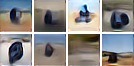
\includegraphics[width=0.23\textwidth]{figures/new/a-rider-on-a-blue-motorcycle-in-the-desert-sharp.png}}\quad
%
\subfloat[\hlcthree{A} rider \hlcone{on} a blue \hlcone{motorcycle} in the \underline{\hlctwo{forest}}.
]{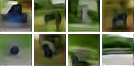
\includegraphics[width=0.23\textwidth]{figures/new/a-rider-on-a-blue-motorcycle-in-the-forest-sharp.png}}\quad
%
\subfloat[\hlctwo{A} \hlcone{surfer}, a woman, and a child walk on the \underline{\hlctwo{beach}}.
]{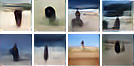
\includegraphics[width=0.23\textwidth]{figures/new/a-surfer-,-a-woman-,-and-a-child-walk-on-the-beach-sharp.png}}\quad
%
\subfloat[\hlcthree{A} \hlcone{surfer}, a woman, and a child walk on the \underline{\hlczero{sun}}.
]{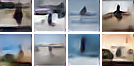
\includegraphics[width=0.23\textwidth]{figures/new/a-surfer-,-a-woman-,-and-a-child-walk-on-the-sun-sharp.png}}\quad
\\
%
\subfloat[alignDRAW]{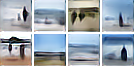
\includegraphics[width=0.23\textwidth]{figures/new/a-group-of-people-walk-on-a-beach-with-surf-boards-sharp-small.png}}\quad
%
\subfloat[LAPGAN]{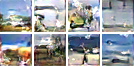
\includegraphics[width=0.23\textwidth]{figures/a-group-of-people-walk-on-a-beach-with-surf-boards-lapgan-small.png}}\quad
%
\subfloat[Conv-Deconv VAE]{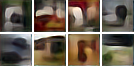
\includegraphics[width=0.23\textwidth]{figures/a-group-of-people-walk-on-a-beach-with-surf-boards-convdeconvvae-small.png}}\quad
%
\subfloat[Fully-Conn VAE]{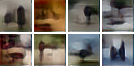
\includegraphics[width=0.23\textwidth]{figures/a-group-of-people-walk-on-a-beach-with-surf-boards-fcvae-small.png}}\quad
%
\end{center}
\caption{\textbf{Bottom}: Four different models displaying results from sampling caption \textit{A group of people walk on a beach with surf boards.} \textbf{Top}: Examples of most attended words while changing the background in the caption.}
\label{fig:diffmodels}
%\vspace{-0.3cm}
\end{figure}

<<<<<<< HEAD
We also tried to analyze the way the model generated images. Unfortunately, we found that there was no significant connection between the patches drawn on canvas and the most attended words at particular time-steps.

\subsubsection{Comparison With Other Models}
Quantitatively evaluating generative models remains a challenging task in of itself as each method of evaluation suffers from its own specific drawbacks. Compared to reporting classification accuracies in discriminative models, the measures defining generative models are intractable most of the times and might not correctly define the real quality of the model. To get a better comparison between performances of different generative models, we report results on two different metrics as well as a qualitative comparison of different generative models.

We compared the performance of the proposed model to the DRAW model conditioned on captions without align function (noalignDRAW) as well as the DRAW model conditioned on skipthought vectors \citep{kiros_skipthought} (skipthoughtDRAW). All of the conditional DRAW models were trained with binary cross-entropy cost function. We also compared our model with Fully-Connected (Fully-Conn) and Convolutional-Deconvolutional (Conv-Deconv) Variational Autoencoders which were trained with the least squares cost function. The LAPGAN model was trained on a two level Laplacian Pyramid with a GAN as a top layer generator and all stages were conditioned on the same skipthought vector.

In Figure~\ref{fig:diffmodels}, we generated several samples from the prior of each of the current state-of-the-art generative models, conditioned on the caption ``A group of people walk on a beach with surf boards". While all of the samples look sharp, the images generated by LAPGAN look more noisy and it is harder to make out definite objects, whereas the images generated by variational models trained with least squares cost function have a watercolor effect on the images. We also found that the quality of generated samples was very similar among different variants of conditional DRAW models.

As for the quantitative comparison of different models, we first compare the performances of the model trained with variational methods. We rank the images in the test set conditioned on the captions based on the variational lower bound of likelihood and then report the Precision-Recall metric as an evaluation of the quality of the generative model (see Table~\ref{tab:results}.). Unsurprisingly, generative models didn't perform well in the image retrieval task. To deal with the large computational complexity involved in looping through each test image, we create a shortlist of one hundred images including the correct one, based on the images having the closest distance in the convolutional feature-space of a VGG-like model \citep{simonyan_convnet} trained on the CIFAR dataset\footnote{The architecture of the model is described here \url{http://torch.ch/blog/2015/07/30/cifar.html}. The shortlist of test images used for evaluation can be downloaded here \url{http://www.cs.toronto.edu/~emansim/cap2im/test-nns.pkl}.} \citep{krizhevsky_cifar}. 
Since there are ``easy'' images for which the model assigns high likelihood independent of the query caption, we look at the ratio of the likelihood of the image conditioned on the sentence to the likelihood of the image conditioned on the mean sentence representation in the training set \citep{kiros_captions}.
We found that the lower bound of log likelihood decreased for sharpened images, and that sharpening considerably hurt the retrieval results. Since sharpening changes the statistics of images, computing reconstruction error for each pixel is not necessarily a good metric.

Instead of calculating error per pixel, we turn to a smarter metric, the Structural Similarity Index (SSI) \citep{wang_ssi}, which incorporates luminance and contrast masking into the error calculation. Strong inter-dependencies of closer pixels are also taken into account and the metric is calculated on small windows of the images. Due to independence property of test captions, we sampled fifty images from the prior of each generative model for every caption in the test set in order to calculate SSI. As you can see on Table~\ref{tab:results}, SSI scores achieved by variational models were higher compared to SSI score achieved by LAPGAN.
%As for another metric of image similarity, we calculated euclidian distance between generated images and real images in the feature space of VGG-like model trained on CIFAR dataset. This is not necessarily a good metric, since the statistics of generated images were vastly different from statistics of training images. Nevertheless, the results are reported on Table~\ref{tab:results}.

% \begin{table}[!t]
% \begin{center}
% \begin{tabulary}{\linewidth}{c || c c c c c || c}
% \hline
% \multicolumn{7}{c}{\textbf{COCO (before sharpening)}} \\
% \hline
% & \multicolumn{5}{c||}{Image Search} & Image Similarity \\
% %\cline{2-6}
% \textbf{Model} & \textbf{R@1} & \textbf{R@5} & \textbf{R@10} & \textbf{R@50} & \textbf{Med r} & \textbf{SSI} \\
% \hline
% \hline
% LAPGAN & - & - & - & - & - & 0.08 \\ % - & - & - & - & - & 0.08
% \hline
% Fully-conn. VAE (L2 cost) & 0.7 & 4.6 & 8.7 & 46.8 & 54 & 0.122 \\ % 0.688 & 4.58 & 8.74 & 46.832 & 54 & -1
% Conv. VAE (L2 cost) & 0.7 & 4.4 & 8.5 & 46.6 & 54 & \textbf{0.131} \\ % 0.672 & 4.448 & 8.476 & 46.596 & 54 & 0.131
% Noalign DRAW & \textbf{1.0} & 6.1 & 11.2 & 52.1 & \textbf{48} & 0.114 \\ % 1.0 & 6.124 & 11.18 & 52.112 & 48 & 0.114
% Skipthought DRAW & \textbf{1.0} & \textbf{6.2} & \textbf{11.5} & \textbf{52.5} & \textbf{48} & 0.118 \\ % 0.988 & 6.18 & 11.48 & 52.512 & 48 & 0.118
% Align DRAW & 0.9 & \textbf{6.2} & 11.2 & \textbf{52.5} & \textbf{48} & 0.115 \\ % 0.924 & 6.216 & 11.184 & 52.492 & 48 & 0.115
% \end{tabulary}
% \end{center}
% \end{table}

\section{Discussion}

In this paper, we demonstrated that the alignDRAW model, a combination of a recurrent variational autoencoder with an alignment model over words, succeeded in generating images that correspond to a given input caption. By extensively using attentional mechanisms, our model gained several advantages. Namely, the use of the visual attention mechanism allowed us to decompose the problem of image generation into a series of steps instead of a single forward pass, while the attention over words provided us an insight whenever our model failed to generate a relevant image. Additionally, our model generated images corresponding to captions which generalized beyond the training set, such as sentences describing novel scenarios which are highly unlikely to occur in real life.

Because the alignDRAW model tends to output slightly blurry samples, likely due to underfitting on the training data, we augmented the model with a sharpening post-processing step in which GAN generated edges which were added to the alignDRAW samples. Unfortunately, this is not an ideal solution due to the fact that the whole model was not trained in an end-to-end fashion. Therefore a direction of future work would be to find methods that can bypass the separate post-processing step and output sharp images directly in an end-to-end manner. 

%\newpage
\section{Acknowledgements}
\begin{table}[!t]
\begin{center}
\begin{tabulary}{\linewidth}{c || c c c c c || c c}
\hline
\multicolumn{7}{c}{\textbf{Microsoft COCO (before sharpening)}} \\
\hline
& \multicolumn{5}{c||}{Image Search} & \multicolumn{1}{c}{Image Similarity} \\
%\cline{2-6}
\textbf{Model} & \textbf{R@1} & \textbf{R@5} & \textbf{R@10} & \textbf{R@50} & \textbf{Med r} & \textbf{SSI}\\ %& \textbf{Feature Distance} \\
\hline
\hline
LAPGAN & - & - & - & - & - & 0.08 \\ % & 6.89 \\ % - & - & - & - & - & 0.08
\hline
Fully-Conn VAE & 1.0 & 6.6 & 12.0 & 53.4 & 47 & 0.156 \\ %& 6.11 \\ % 0.688 & 4.58 & 8.74 & 46.832 & 54 & -1
Conv-Deconv VAE & 1.0 & 6.5 & 12.0 & 52.9 & 48 & 0.164 \\ %& 6.32 \\ % 0.672 & 4.448 & 8.476 & 46.596 & 54 & 0.131
skipthoughtDRAW & 2.0 & 11.2 & 18.9 & 63.3 & 36 & 0.157 \\ %& 6.93 \\ % 0.988 & 6.18 & 11.48 & 52.512 & 48 & 0.118
noalignDRAW & 2.8 & 14.1 & 23.1 & 68.0 & 31 & 0.155 \\ %& 7.01 \\ % 1.0 & 6.124 & 11.18 & 52.112 & 48 & 0.114
alignDRAW & 3.0 & 14.0 & 22.9 & 68.5 & 31 & 0.156 \\ %& 6.99 \\ % 0.924 & 6.216 & 11.184 & 52.492 & 48 & 0.115
\end{tabulary}
\end{center}
\caption{Results of different models.}
\label{tab:results}
%\vspace{-0.3cm}
\end{table}
We would like to thank developers of Theano \citep{theano} for a powerful software and authors of \citep{denton_lapgan} for open sourcing their code. We would also like to thank Ryan Kiros and Nitish Srivastava for helpful discussions. We will be releasing our code with pretrained models.

\bibliography{iclr-paper}
\bibliographystyle{iclr-style/iclr2016_conference}

\newpage
\appendix


\section*{Appendix A: MNIST With Captions}

\begin{figure}[!t]
\captionsetup[subfigure]{labelformat=empty}
\begin{center}
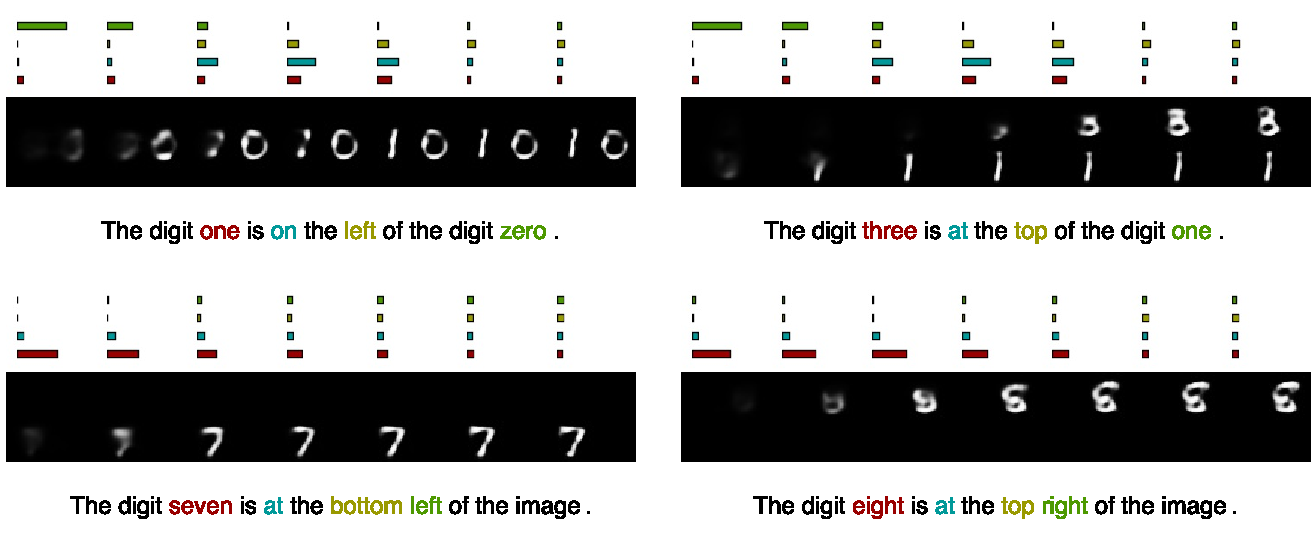
\includegraphics[width=0.99\textwidth]{figures/new/mnist/test3.pdf}\quad
%
\end{center}
\caption{Examples of generating $60 \times 60$ MNIST images corresponding to respective captions. The captions on the \textbf{left column} were part of the training set. The digits described in the captions on the \textbf{right column} were hidden during training for the respective configurations.}
\label{fig:figmnist}
\vspace{-0.3cm}
\end{figure}

As an additional experiment, we trained our model on the MNIST dataset with artificial captions. Either one or two digits from the MNIST training dataset were placed on a $60 \times 60$ blank image. One digit was placed in one of the four (top-left, top-right, bottom-left or bottom-right) corners of the image. Two digits were either placed horizontally or vertically in nonoverlapping fashion. The corresponding artificial captions specified the 
identity of each digit along with their relative positions, e.g. ``The digit two is on the top  
of the digit zero'', or ``The digit seven is at the bottom left of the image''.  

The generated images together with the attention alignments are displayed in Figure~\ref{fig:figmnist}. The model correctly displayed the specified digits at the described positions and even managed to generalize 
reasonably well to the configurations that were never present during training.
In the case of generating two digits, the model would dynamically attend 
to the digit in the caption it was drawing at that particular time-step. 
Similarly, in the setting where the caption specified only a single digit, the model would correctly 
attend to the digit in the caption during the whole generation process. 
In both cases, the model placed small attention values on the words describing the position of digits in the images.

\section*{Appendix B: Training Details}
\label{sec:training_details}

\subsection*{Hyperparameters}

Each parameter in alignDRAW was initialized by sampling from a Gaussian distribution with 
mean $0$ and standard deviation $0.01$. The model was trained using \textit{RMSprop} with an initial learning rate of $0.001$. The norm of the gradients was clipped at a maximum of $10.0$ during training to deal with exploding gradients. We used a vocabulary size of $K = 25323$ and $K = 22$ for Microsoft COCO and MNIST with Captions respectively. All capital letters in the words were converted to small letters as a preprocessing step. For all tasks, $\overrightarrow{h}^{lang}_{n}$ and $\overleftarrow{h}^{lang}_{n}$ in the language model had $128$ units. The parameters in the \textit{align} operator had a dimensionality of $l = 512$, $\vv \in \mathbb{R}^{512}$, $U \in \mathbb{R}^{512 \times 128}$, $W \in \mathbb{R}^{512 \times n^{gen}}$ and $b \in \mathbb{R}^{512}$. For the Microsoft COCO task, the alignDRAW model was trained for $18$ epochs and the learning rate was reduced by the factor of $0.1$ after $11$ epochs. The architectural configurations of alignDRAW models are shown on Table~\ref{tab:drawhyper}.

\begin{table}[!t]
\begin{center}
\begin{tabulary}{\linewidth}{c | c c c c c c}
\hline
\multicolumn{7}{c}{\textbf{alignDRAW Model}} \\
\hline
Task & \#glimpses & Inference \#$h$ & Generative \#$h$ & \#$z$ & Read Size & Write Size\\
\hline
Microsoft COCO & 32 & 550 & 550 & 275 & 9 & 9\\
MNIST Captions & 32 & 300 & 300 & 150 & 8 & 8\\
\end{tabulary}
\caption{The architectural configurations of alignDRAW models.}
\label{tab:drawhyper}
\end{center}
%\vspace{-0.3cm}
\end{table}

The GAN model used for sharpening had the same configuration as the $28 \times 28$ model trained by \cite{denton_lapgan} on the edge residuals of the CIFAR dataset. The configuration can be found at \url{https://gist.github.com/soumith/e3f722173ea16c1ea0d9}. The model was trained for $6$ epochs. 
For the LAPGAN model, we used a data augmentation step where we took 5 crops (top-left, top-right, bottom-left, bottom-right, center) of a downsampled COCO image and assigned each crop one of the 5 captions that described the uncropped image.

\subsection*{Evaluation}

Table~\ref{tab:nll} shows the estimated variational lower bound on the average train/validation/test 
log-probabilities.
Note that the alignDRAW model does not suffer much from overfitting. 
The results worsened dramatically after sharpening test images.

\begin{table}[!h]
\begin{center}
\begin{tabulary}{\linewidth}{c | c c c c}
\hline
Model & Train LL & Valid LL & Test LL & Test LL (after sharpening)\\
\hline
skipthoughtDRAW & -1794.29 & -1797.41 & -1791.37 & -2045.84 \\
noalignDRAW & -1792.14 & -1796.94 & -1791.15 & -2051.07 \\
alignDRAW & -1792.15 & -1797.24 & -1791.53 & -2042.31
\end{tabulary}
\caption{The lower bound on the average test log-probabilities of conditional DRAW models, trained on the Microsoft COCO dataset.}
\label{tab:nll}
\end{center}
\end{table}

\newpage
\section*{Appendix C: Effect of Sharpening Images.}
\label{sec:post_processing}

\begin{figure}[!h]
\captionsetup[subfigure]{labelformat=empty}
\vspace{-0.27in}
\begin{center}
\subfloat[]{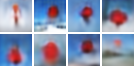
\includegraphics[width=0.23\textwidth]{figures/new/a-stop-sign-is-flying-in-blue-skies-blurry.png}}\quad
%
\subfloat[]{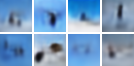
\includegraphics[width=0.23\textwidth]{figures/new/a-herd-of-elephants-flying-in-the-blue-skies-blurry.png}}\quad
%
\subfloat[]{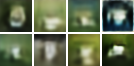
\includegraphics[width=0.23\textwidth]{figures/new/a-toilet-seat-sits-open-in-the-grass-field-blurry.png}}\quad
%
\subfloat[]{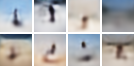
\includegraphics[width=0.23\textwidth]{figures/new/a-person-skiing-on-sand-clad-vast-desert-blurry.png}}\\
\vspace{-0.45cm}
%
\subfloat[%A stop sign is flying in blue skies.
]{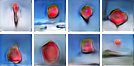
\includegraphics[width=0.23\textwidth]{figures/new/a-stop-sign-is-flying-in-blue-skies-sharp.png}}\quad
%
\subfloat[%A herd of elephants flying in the blue skies.
]{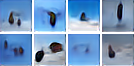
\includegraphics[width=0.23\textwidth]{figures/new/a-herd-of-elephants-flying-in-the-blue-skies-sharp.png}}\quad
%
\subfloat[%A toilet seat sits open in the grass field.
]{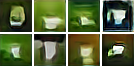
\includegraphics[width=0.23\textwidth]{figures/new/a-toilet-seat-sits-open-in-the-grass-field-sharp.png}}\quad
%
\subfloat[%A person skiing on sand clad vast desert.
]{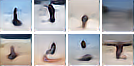
\includegraphics[width=0.23\textwidth]{figures/new/a-person-skiing-on-sand-clad-vast-desert-sharp.png}}\\
%

\subfloat[]{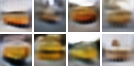
\includegraphics[width=0.23\textwidth]{figures/new/a-yellow-school-bus-parked-in-a-parking-lot-blurry.png}}\quad
%
\subfloat[]{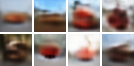
\includegraphics[width=0.23\textwidth]{figures/new/a-red-school-bus-parked-in-a-parking-lot-blurry.png}}\quad
%
\subfloat[]{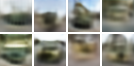
\includegraphics[width=0.23\textwidth]{figures/new/a-green-school-bus-parked-in-a-parking-lot-blurry.png}}\quad
%
\subfloat[]{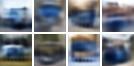
\includegraphics[width=0.23\textwidth]{figures/new/a-blue-school-bus-parked-in-a-parking-lot-blurry.png}}\\
\vspace{-0.45cm}
%
\subfloat[%A yellow school bus parked in a parking lot.
]{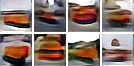
\includegraphics[width=0.23\textwidth]{figures/new/a-yellow-school-bus-parked-in-a-parking-lot-sharp.png}}\quad
%
\subfloat[%A red school bus parked in a parking lot.
]{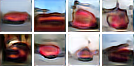
\includegraphics[width=0.23\textwidth]{figures/new/a-red-school-bus-parked-in-a-parking-lot-sharp.png}}\quad
%
\subfloat[%A green school bus parked in a parking lot.
]{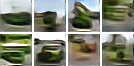
\includegraphics[width=0.23\textwidth]{figures/new/a-green-school-bus-parked-in-a-parking-lot-sharp.png}}\quad
%
\subfloat[%A blue school bus parked in a parking lot.
]{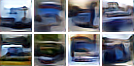
\includegraphics[width=0.23\textwidth]{figures/new/a-blue-school-bus-parked-in-a-parking-lot-sharp.png}}\\
%

\subfloat[]{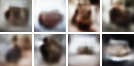
\includegraphics[width=0.23\textwidth]{figures/new/the-decadent-chocolate-dessert-is-on-the-table-blurry.png}}\quad
%
\subfloat[]{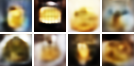
\includegraphics[width=0.23\textwidth]{figures/new/a-bowl-of-bananas-is-on-the-table-blurry.png}}\quad
%
\subfloat[]{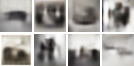
\includegraphics[width=0.23\textwidth]{figures/new/a-vintage-photo-of-a-cat-blurry.png}}\quad
%
\subfloat[]{\includegraphics[width=0.23\textwidth]{figures/new/a-vintage-photo-of-a-dog-blurry.png}}\\
\vspace{-0.45cm}
%
\subfloat[%The decadent chocolate desert is on the table.
]{\includegraphics[width=0.23\textwidth]{figures/new/the-decadent-chocolate-dessert-is-on-the-table-sharp.png}}\quad
%
\subfloat[%A bowl of bananas is on the table.
]{\includegraphics[width=0.23\textwidth]{figures/new/a-bowl-of-bananas-is-on-the-table-sharp.png}}\quad
%
\subfloat[%A vintage photo of a cat.
]{\includegraphics[width=0.23\textwidth]{figures/new/a-vintage-photo-of-a-cat-sharp.png}}\quad
%
\subfloat[%A vintage photo of a dog.
]{\includegraphics[width=0.23\textwidth]{figures/new/a-vintage-photo-of-a-dog-sharp.png}}\\
%

\subfloat[]{\includegraphics[width=0.23\textwidth]{figures/new/a-very-large-commercial-plane-flying-in-blue-skies-blurry.png}}\quad
%
\subfloat[]{\includegraphics[width=0.23\textwidth]{figures/new/a-very-large-commercial-plane-flying-in-rainy-skies-blurry.png}}\quad
%
\subfloat[]{\includegraphics[width=0.23\textwidth]{figures/new/a-herd-of-elephants-walking-across-a-dry-grass-field-blurry.png}}\quad
%
\subfloat[]{\includegraphics[width=0.23\textwidth]{figures/new/a-herd-of-elephants-walking-across-a-green-grass-field-blurry.png}}\\
\vspace{-0.45cm}
%
\subfloat[%A very large commercial plane flying in blue skies.
]{\includegraphics[width=0.23\textwidth]{figures/new/a-very-large-commercial-plane-flying-in-blue-skies-sharp.png}}\quad
%
\subfloat[%A very large commercial plane flying in rainy skies.
]{\includegraphics[width=0.23\textwidth]{figures/new/a-very-large-commercial-plane-flying-in-rainy-skies-sharp.png}}\quad
%
\subfloat[%A herd of elephants walking across a dry grass field.
]{\includegraphics[width=0.23\textwidth]{figures/new/a-herd-of-elephants-walking-across-a-dry-grass-field-sharp.png}}\quad
%
\subfloat[%A herd of elephants walking across a green grass field.
]{\includegraphics[width=0.23\textwidth]{figures/new/a-herd-of-elephants-walking-across-a-green-grass-field-sharp.png}}\\
%

\subfloat[]{\includegraphics[width=0.23\textwidth]{figures/new/a-rider-on-a-blue-motorcycle-in-the-desert-blurry.png}}\quad
%
\subfloat[]{\includegraphics[width=0.23\textwidth]{figures/new/a-rider-on-a-blue-motorcycle-in-the-forest-blurry.png}}\quad
%
\subfloat[]{\includegraphics[width=0.23\textwidth]{figures/new/a-surfer-,-a-woman-,-and-a-child-walk-on-the-beach-blurry.png}}\quad
%
\subfloat[]{\includegraphics[width=0.23\textwidth]{figures/new/a-surfer-,-a-woman-,-and-a-child-walk-on-the-sun-blurry.png}}\\
\vspace{-0.45cm}
%
\subfloat[%A rider on a blue motorcycle in the desert.
]{\includegraphics[width=0.23\textwidth]{figures/new/a-rider-on-a-blue-motorcycle-in-the-desert-sharp.png}}\quad
%
\subfloat[%A rider on a blue motorcycle in the forest.
]{\includegraphics[width=0.23\textwidth]{figures/new/a-rider-on-a-blue-motorcycle-in-the-forest-sharp.png}}\quad
%
\subfloat[%A surfer, a woman, and a child walk on the beach.
]{\includegraphics[width=0.23\textwidth]{figures/new/a-surfer-,-a-woman-,-and-a-child-walk-on-the-beach-sharp.png}}\quad
%
\subfloat[%A surfer, a woman, and a child walk on the sun.
]{\includegraphics[width=0.23\textwidth]{figures/new/a-surfer-,-a-woman-,-and-a-child-walk-on-the-sun-sharp.png}}\\
\end{center}
%
%\caption{\small Effect of sharpening generated images shown in the publication \textbf{Bottom}: Sharpened Images. \textbf{Top}: Original Images}
%\vspace{-0.1in}
\end{figure}


\end{document}
